\documentclass[12pt,italian]{report}
\usepackage{tesi}

%
%			INFORMAZIONI SULLA TESI
%			DA COMPILARE!
%

% CORSO DI LAUREA:
\def\myCDL{Corso di Laurea triennale in\\Informatica}

% TITOLO TESI:
\def\myTitle{ANALISI DEI DATI PER PROBLEMI DI MEDICINA LEGALE}

% AUTORE:
\def\myName{Alessandro Beranti}
\def\myMat{Matr. Nr. 855489}

% RELATORE E CORRELATORE:
\def\myRefereeA{Prof. Dario Malchiodi}
\def\myRefereeB{Prof. Anna Maria Zanaboni}

% ANNO ACCADEMICO
\def\myYY{2018-2019}

% Il seguente comando introduce un elenco delle figure dopo l'indice (facoltativo)
%\figurespagetrue

% Il seguente comando introduce un elenco delle tabelle dopo l'indice (facoltativo)
%\tablespagetrue

%
%			PREAMBOLO
%			Inserire qui eventuali package da includere o definizioni di comandi personalizzati
%

% Package di formato
\usepackage[a4paper]{geometry}		% Formato del foglio
\usepackage[italian]{babel}			% Supporto per l'italiano
\usepackage[utf8]{inputenc}			% Supporto per UTF-8
%\usepackage[a-1b]{pdfx}			% File conforme allo standard PDF-A (obbligatorio per la consegna)

% Package per la grafica
\usepackage{graphicx}				% Funzioni avanzate per le immagini
\usepackage{hologo}					% Bibtex logo with \hologo{BibTeX}
%\usepackage{epsfig}				% Permette immagini in EPS
%\usepackage{xcolor}				% Gestione avanzata dei colori

% Package tipografici
\usepackage{amssymb,amsmath,amsthm} % Simboli matematici
\usepackage{listings}				% Scrittura di codice

% Package ipertesto
\usepackage{url}					% Visualizza e rendere interattii gli URL
\usepackage{hyperref}				% Rende interattivi i collegamenti interni

\usepackage{verbatim}

\setcounter{tocdepth}{4}
\setcounter{secnumdepth}{4}
\begin{document}

% Creazione automatica del frontespizio
\frontespizio
\beforepreface

% 
%			PAGINA DI DEDICA E/O CITAZIONE
%			facoltativa, questa è l'unica cosa che dovete formattare a mano, un po' come vi pare
%

{\raggedleft \large \sl Questo lavoro \`{e} dedicato a tutti gli studenti\\
	
	\vspace{2cm}
	
	``Io studio,\\ma studiate pure voi,\\che se studio solo io non serve a un c\dots o''
	
	\bigskip
	
	\--- Gli scarabocchi di Maicol \& Mirco\\
  
	\vspace{2cm}
	
	``No tale is so good \\ that it can't be spoiled \\ in the telling''
	
	\bigskip
	
	\--- Proverbio\\}
         
% 
%			PREFAZIONE (facoltativa)
%

%\prefacesection{Prefazione}
%Le prefazioni non sono molto comuni, tuttavia a volte capita che qualcuno voglia dire qualcosa che esuli dal lavoro in s\'e (come un meta-commento sull'elaborato), o voglia fornire informazioni riguardanti l'eventuale progetto entro cui la tesi si colloca (in questo caso \`e probabile che sia il relatore a scrivere questa parte).

%
%			RINGRAZIAMENTI (facoltativi)
%

\prefacesection{Ringraziamenti}
Questa sezione, facoltativa, contiene i ringraziamenti.

%
%			Creazione automatica dell'indice
%

\afterpreface

% 
%			CAPITOLO 1: Introduzione o Abstract
% 

\chapter{Introduzione}
\label{cap:introduzione}

Questo documento ha una duplice funzione: da un lato mostra un esempio completo di elaborato finale redatto in \LaTeX\ e conforme allo standard PDF/A, e dall'altro contiene suggerimenti e risposte a domande frequenti poste dagli studenti. Se ne raccomanda, pertanto, un'attenta lettura.

\chapter{Machine Learning}
Il termine Machine Learning, o apprendimento automatico in italiano, si riferisce alla capacità dei computer di apprendere e agire senza essere programmati esplicitamente.
Gli strumenti di machine learning si occupano di dotare i programmi della capacità di ``apprendere'' e adattarsi agli input forniti.
Al giorno d'oggi siamo circondati da tecnologie basate sull'apprendimento automatico:
\begin{itemize}
	\item software che rilevano lo spam a partire dai nostri messaggi e-mail  
	\item i motori di ricerca che imparano a fornirci i migliori risultati possibili
	\item le transazioni con carta di credito protette da un software che impara a rilevare le frodi
	\item le fotocamere digitali imparano a rilevare i volti
	\item le applicazioni di assistenza personale intelligenti sugli smartphone imparano a riconoscere i comandi vocali
	\item addestramento dei veicoli per guidare senza intervento umano
	\item applicazioni scientifiche come la bioinformatica, la medicina e l'astronomia
\end{itemize}
\section{Come funziona il Machine Learning}
\label{sec:Come funziona il Machine Learning}
Nel Machine Learning vengono usati metodi statistici che utilizzano l'esperienza per migliorare le prestazioni di algoritmi o fare previsioni più accurate.
La qualità e la dimensione dei dataset (collezione di dati), raccolti o resi disponibili e utilizzati nel processo sono fondamentali per il successo e l'accuratezza delle previsioni fatte.

Nel processo possiamo distinguere diversi aspetti:
\begin{itemize}
	\item Domain set: raccolta arbitraria di dati, X. Questo è l'insieme di oggetti che si desidera etichettare
	\item Label set: generalmente si usa un set di etichette del tipo \{0, 1\} che rappresentano la presenza o l'assenza della caratteristica che si sta cercando
	\item Training data: è l'input dato in pasto al computer
	\item Algoritmo: scelto in base ai dati in input, è la regola che viene usata dal sistema per classificare e in generale predire la caratteristica
	\item Errore di generalizzazione: è la probabilità che non venga predetta l'etichetta corretta 
\end{itemize}
Una categorizzazione dei compiti del machine learning si ha quando si considera l'output desiderato del sistema che può essere di diversi tipi:
\begin{itemize}
	\item classificazione, i classificatori separano i dati in due o più classi. Quando fornisco un esempio al classificatore, l'algoritmo mi restituisce la classe a cui potrebbe appartenere.
	Esistono due tipi di classificazione:
	\begin{itemize}
		\item binaria: le etichette sono soltanto due
		\item multiclasse: le etichette sono tre o più
	\end{itemize}
	\item regressione, usata per predire un valore continuo, per esempio il prezzo di una casa date la dimensione e metratura
	\item clustering, un insieme di input viene diviso in gruppi in modo che i singoli elementi siano simili agli altri punti dello stesso insieme e diversi dagli elementi degli altri. Diversamente da quanto accade per la classificazione, i gruppi non sono noti prima, rendendolo tipicamente un compito non supervisionato.
\end{itemize}
I compiti dell'apprendimento automatico vengono tipicamente classificati in quattro categorie, a seconda della natura del ``segnale'' utilizzato per l'apprendimento o del ``feedback'' disponibile al sistema di apprendimento. Queste categorie, anche dette paradigmi, sono:
\begin{itemize}
	\item Machine Learning supervisionato
	\item Machine Learning non supervisionato
	\item Machine Learning per rinforzo
	\item Machine Learning semi-supervisionato
	
\end{itemize}

\subsection{Machine Learning con apprendimento \\supervisionato}
\label{sec:apprendimento supervisionato}
Attraverso l’apprendimento supervisionato cerchiamo di costruire un modello partendo da dati di addestramento etichettati, con i quali cerchiamo di fare previsioni su dati non disponibili o futuri. Con il termine ``supervisione'' si intende quindi che nel nostro insieme dei campioni (o dataset), i segnali di output desiderati sono già noti poiché precedentemente etichettati.

Esistono molti algoritmi per svolgere apprendimento supervisionato, durante il tirocinio ho avuto modo di usare:
\begin{itemize}
	\item Support Vector Machine
	\item Decison Tree Classifier
	\item Random Forest Classifier
	\item Gaussian Naive Bayes
	\item Linear Discriminant Analysis
	\item Multi-Layer Perceptron Classifier
\end{itemize}

\subsubsection{Support Vector Machine}
\label{sec:SVC}
Il Support Vector Machine è un algoritmo di apprendimento automatico supervisionato che può essere usato sia per scopi di classificazione che di regressione, ha la sua massima efficacia in problemi di classificazione binaria anche se può essere utilizzato anche per problemi di classificazione multiclasse.

L'SVM è basato sull'idea di riuscire a trovare un iperpiano che divida al meglio un set di elementi in due classi distinte, definiamo alcuni concetti chiave:


\begin{itemize}
	\item Iperpiano: nel caso in cui si abbiano solo due dimensioni spaziali $x_1$ e $x_2$, l'iperpiano è raffigurato come una linea che separa un insieme di dati. Nel caso in cui le dimensioni siano 3, l'iperpiano è raffigurato come un piano, vedi figura 1.
	\begin{figure}[h]
		\centering
		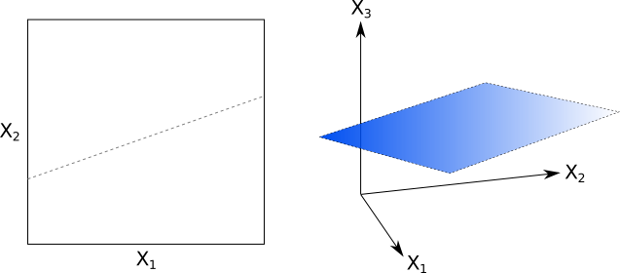
\includegraphics[width = 50mm]{immagini/Iperpiano-3-dimensioni}
		\caption{Iperpiano in 3 dimensioni}
	\end{figure}
	Con più di 3 dimensioni viene definito ``iperpiano''.
	\item Support Vector: chiamati vettori di supporto in italiano, sono i punti che si trovano piu vicini all'iperpiano che divide i dati.
	\item Margine: è la distanza tra i vettori di supporto di due classi diverse. A metà di questa distanza viene tracciato l'iperpiano, vedi figura 2.
\end{itemize}

\begin{figure}[h]
	\centering
	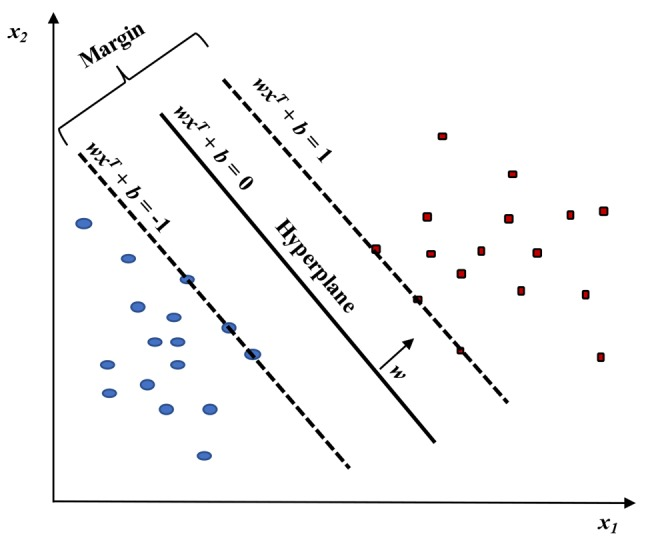
\includegraphics[width = 47mm]{immagini/svc}
	\caption{Margine e vettori di supporto}
\end{figure}

Il Support Vector Machine ha l'obiettivo di identificare l'iperpiano che divide meglio i vettori di supporto in classi, per fare ciò esegue due step:

\begin{itemize}
	\item cerca un iperpiano linearmente separabile che separa i valori di una classe dall'altra. Nel caso in cui ne esista più di uno cerca quello con il margine più alto tra i vettori di supporto in modo da migliorare l'accuratezza del modello.
	\item se l'iperpiano cercato non esiste, Support Vector Machine usa una mappatura non lineare per trasformare i dati di allenamento in una dimensione superiore. In questo modo, i dati di due classi possono sempre essere separati da un iperpiano, che sarà scelto per la suddivisione dei dati.
\end{itemize}

Un iperpiano linearmente separabile è un iperpiano in cui è semplice distinguere due classi. Nella figura 3 è visibile come sia possibile disegnare un numero infinito di linee rette per separare i diversi elementi. Il problema è trovare quale tra le infinite rette risulti ottimale, ossia quella che generi il minimo errore di classificazione su una nuova osservazione.
Per fare ciò dobbiamo avere i nostri elementi il più lontano possibile dall' iperpiano pur rimanendo nella zona corretta. 
\begin{figure}[h]
	\centering
	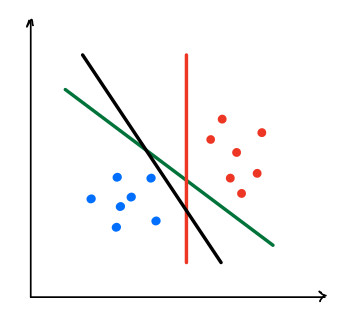
\includegraphics[width = 40mm]{immagini/linearmente-separabili}
	\caption{Infinite rette possono separare gli elementi}
\end{figure}

Nel momento in cui vengono aggiunti nuovi dati di test, il modello decide la classe che gli appartiene.

Dato un training set etichettato:

\begin{center}
	\[
	\ (x_1, y_1), ..., (x_n, y_n) \in R^{d} and 
	\ y_i \in (-1, +1)
	\]
\end{center}
dove $x_i$ sono le dimensioni del vettore e $y_i$ sono le etichette.

L'iperpiano ottimale è definito come 
\begin{center}
	\[w_0 + w_1x_1 + w_2x_2 +...+ w_nx_n= 0\]
\end{center}
dove w è il vettore di peso, x è il vettore di caratteristiche di input e $w_0$ è il bias.
In sostanza in $n$ dimensioni un iperpiano di separazione è una combinazione lineare di tutte le dimensioni uguagliate a 0.
Ragionando a due dimensioni per semplificare il problema abbiamo che 
\begin{center}
	\[w_0 + w_1x_1 + w_2x_2 = 0\]
\end{center}
I punti che stanno sopra l'iperpiano e che rappresentano un classe soddisfano la seguente condizione:
\begin{center}
	\[w_0 + w_1x_1+w_2x_2 > 0\]
\end{center}
mentre qualsiasi punto che si trova sotto l'iperpiano, appartiene all'altra classe, che è soddisfatta dalla seguente condizione :
\begin{center}
	\[w_0 + w_1x_1+w_2x_2 < 0\]
\end{center}
Includendo anche i limiti dei margini delle classi si hanno le seguenti condizioni:
\begin{center}
	\[w_0 + w_1x_1+w_2x_2 \geq 1,
	\ if
	\ y=1\]
	\[
	\ w_0 + w_1x_1+w_2x_2 \leq 1 
	\ if
	\ y = -1
	\]
	\[ y \in (-1, +1)\]
\end{center}
Se il vettore dei pesi è indicato da $w$ e $\parallel w \parallel$ è la sua lunghezza, allora la dimensione del margine massimo è 
\begin{center}
	\[ \frac{1}{\left | w \right |} + \frac{1}{\left | w \right |} = \frac{2}{\left | w \right |}\]
\end{center}
ciò significa che minimizzando il vettore peso $w$, avremo margine massimo che determina l'iperpiano ottimale.

Non è però sempre possibile dividere i dati tramite un iperpiano, nella figura sotto vi è un chiaro esempio

\begin{figure}[h]
	\centering
	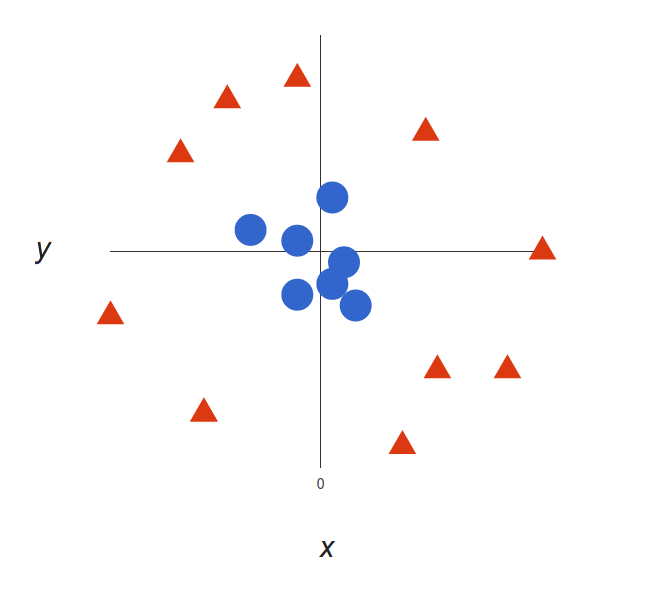
\includegraphics[width = 40mm]{immagini/esempio_dataset_non_lineare}
	\caption{Non sempre è possibile dividere i dati linearmente}
\end{figure}

Per utilizzare la classificazione tramite iperpiani anche per dati che avrebbero bisogno di funzioni non lineari per essere separati, è necessario ricorrere alla tecnica degli spazi immagine ($feature$ $spaces$). Questo metodo, che sta alla base della teoria delle SVM, consiste nel mappare i dati iniziali in uno spazio di dimensione superiore.  Presupponendo quindi $m > n$, per la mappa si utilizza una funzione
\begin{equation}
	\phi: \mathbb{R}^{n} \rightarrow \mathbb{R}^{m}
\end{equation}
attraverso la funzione $\phi$ i dati vengono mappati in uno spazio in cui diventano linearmente separabili e in cui sarà possibile trovare un iperpiano che li separi.

La tecnica degli spazi immagine è particolarmente interessante per algoritmi che utilizzano i dati di training $x_i$ solo attraverso prodotti scalari $x_i \cdot x_j$. In questo caso nello spazio $\mathbb{R}^{m}$ non si devono trovare esplicitamente $\phi(x_i)$ e $\phi (x_j)$ ma basta calcolare il loro prodotto scalare $\phi (x_i) \cdot \phi (x_j)$. Per rendere semplice questo ultimo calcolo, che in spazi di dimensioni elevate diventa molto complicato, si utilizza una funzione detta \textit{kernel} che restituisce direttamente il prodotto scalare delle immagini:
\begin{equation}
K(x_i, x_j) = \phi (x_i) \cdot \phi (x_j)
\end{equation}
Esistono svariati \textit{kernel}, i più utilizzati sono:
\begin{itemize}
	\item Lineare: $K(x, y) = x \cdot y$
	\item Polinomiale: $K(x, y) = (x \cdot y)^{d}$ oppure $K(x, y) = (1 + x \cdot y)^{d}$
	\item Gaussian Radial Basis function: $K(x,y) = exp (- \left | x-y \right |^2)/(2 \sigma 2)$
	\item Sigmoid: $K(x,y) = tanh(k x \cdot y - \delta)$ 
\end{itemize}

\subsubsection{Decision Tree Classifier}
Il Decision Tree Classifier è un algoritmo di apprendimento supervisionato. È un metodo privo di distribuzione o non parametrico, che non dipende da ipotesi di distribuzione di probabilità. Utilizza un albero decisionale, \textit{decision tree}, composto da:
\begin{itemize}
	\item Nodi: rappresenta la caratteristica o attributo
	\item Ramo: rappresenta una regola di decisione
	\item Foglia: rappresenta il risultato
\end{itemize}

Normalmente il decision tree viene costruito a partire dall'insieme dei dati iniziali (data set), il quale può essere diviso in due sottoinsiemi: il \textit{training set}, sulla base del quale si crea la struttura dell'albero, e il \textit{test set} che viene utilizzato per testare l'accuratezza del modello predittivo così creato.
Il processo di partizionamento avviene in maniera ricorsiva. In figura 5 vi è una sua visualizzazione come diagramma di flusso è utile per capire il suo funzionamento
\begin{figure}[h]
	\centering
	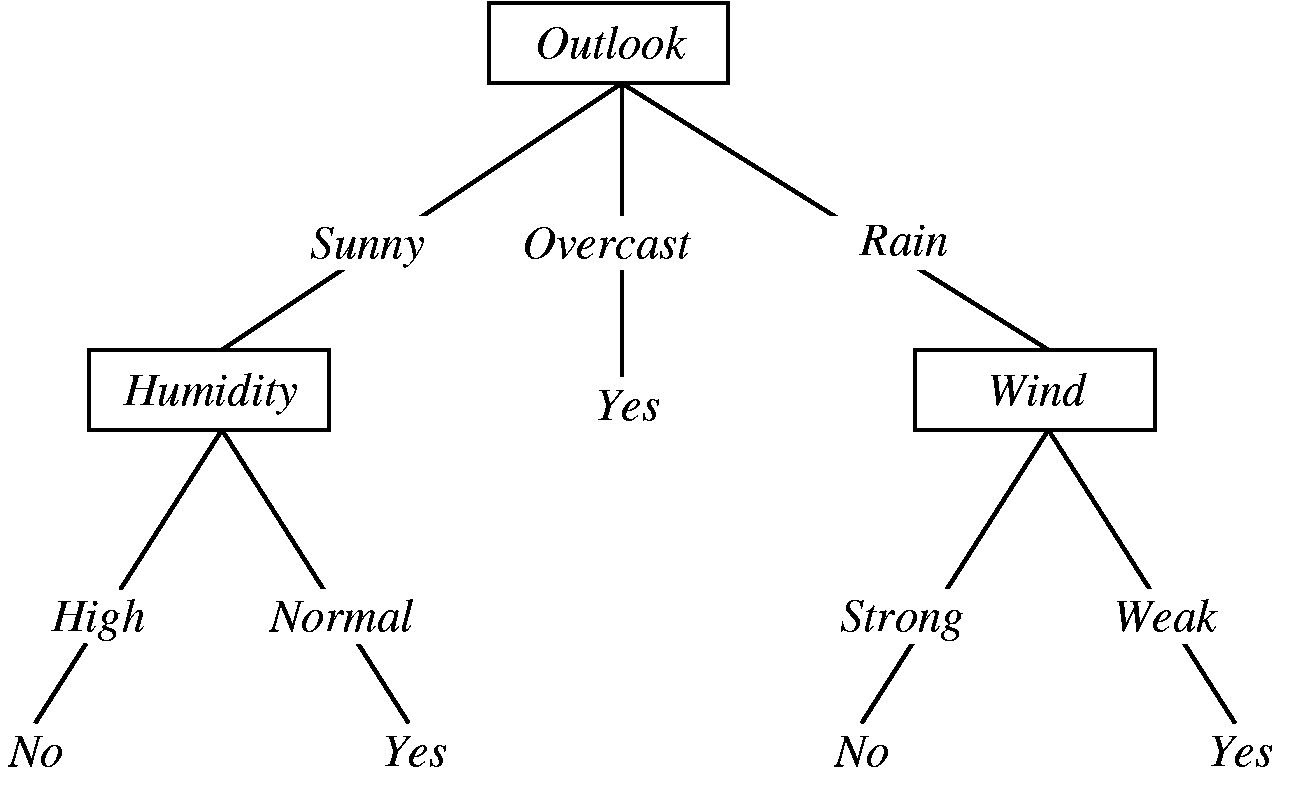
\includegraphics[width = 52mm]{immagini/decision_tree}
	\caption{Visualizzazione decision tree come diagramma di flusso}
\end{figure}

L'algoritmo si compone di tre passaggi:
\begin{itemize}
	\item 1) Seleziona l'attributo migliore utilizzando le misure di selezione degli attributi per dividere i record
	\item 2) Trasforma tale attributo in un nodo decisionale e suddivide il set di dati in sottoinsiemi più piccoli
	\item 3) Inizia la costruzione dell'albero ripetendo questo processo in modo ricorsivo per ogni figlio fino a quando una delle seguenti condizioni non verrà rispettata:
	\begin{itemize}
		\item Tutte le tuple appartengono allo stesso valore di attributo
		\item Non ci sono più attributi rimanenti
		\item Non ci sono più casi
	\end{itemize}
\end{itemize}

La misura di selezione degli attributi è un'euristica per selezionare il criterio di suddivisione che divide i dati nel miglior modo possibile. I più famosi sono l'entropia e l'indice di Gini.
(parlare di loro nel caso ci sia spazio)

\subsubsection{Random Forest Classifier}
Il Random Forest Classifier è un algoritmo di apprendimento supervisionato. Esso si compone di un grande numero di singoli alberi di decisione che operano come un insieme. Ogni albero della foresta genera una previsione e quella che compare più frequentemente diventa la previsione del modello. 

Il concetto fondamentale dietro una foresta casuale risiede nel fatto che un grande numero di alberi non correlati tra loro che operano insieme saranno più efficienti di un singolo albero.

La bassa correlazione è la chiave, modelli non correlati possono produrre previsioni d'insieme più accurate di qualsiasi singola previsione. La ragione risiede nel fatto che, anche se alcuni alberi potrebbero sbagliare, molti altri avranno ottenuto la previsione corretta.
\subsubsection{Gaussian Naive Bayes}
Il Gaussian Naive Bayes è uno dei più semplici algoritmi di apprendimento supervisionato, si basa sul teorema di Bayes. L'algoritmo assume che l'effetto di una particolare caratteristica in una classe sia indipendente dalle altre caratteristiche. Anche se le caratteristiche sono interdipendenti, esse vengono comunque considerate in modo indipendente. Questa ipotesi semplifica il calcolo, ed è per questo che è considerata naive. Questo assunto si chiama indipendenza condizionale di classe.
Usiamo il teorema di Bayes:
\begin{equation}
P(y | X) = \frac{P(X | y) P(y)}{P(X)}
\end{equation}
dove $y$ è l'etichetta e $X = (x_1, x_2, x_3, ..., x_n)$ ovvero il vettore di caratteristiche di lunghezza $n$

Siccome abbiamo assunto che le caratteristiche siano indipendenti possiamo dire che:
\begin{equation}
P(y| x_1,..., x_n) = \frac{P(x_1|y) P(x_2|y)...P(x_n|y)P(y)}{P(x_1)P(x_2)...P(x_n)}
\end{equation}
Poiché il denominatore rimane costante per un determinato input possiamo rimuoverlo e scrivere:
\begin{equation}
P(y| x_1,..., x_n) = P(y) \prod_{i=1}^{n} P(x_1|y)
\end{equation}
Ora dobbiamo creare un modello per classificare. Lo facciamo trovando la probabilità di un dato insieme di input per tutti i possibili valori di y e prendendo l'output con la massima probabilità:
\begin{equation}
y = argmax_y P(y) \prod_{i=1}^{n} P(x_i|y)
\end{equation}
Rimane solo da calcolare $P(y)$ e $P(x_i|y)$ ricavabile dal dataset dato in input al sistema.

Nel Gaussian Naive Bayes si presume che i valori continui associati a ciascuna caratteristica siano distribuiti secondo una distribuzione gaussiana. Una distribuzione gaussiana è anche chiamata distribuzione normale. Una volta tracciato, fornisce una curva a campana simmetrica rispetto alla media dei valori delle caratteristiche, come mostrato in figura qui sotto:

\begin{figure}[h]
	\centering
	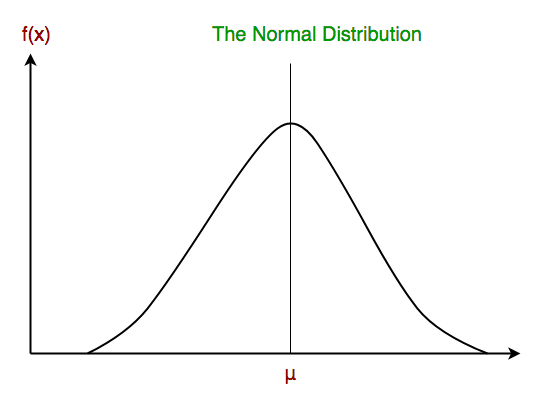
\includegraphics[width = 58mm]{immagini/naive-bayes-classification-1}
	\caption{Distribuzione normale o gaussiana}
\end{figure}

Si presume che la probabilità delle caratteristiche sia gaussiana, quindi la probabilità condizionata è data da:
\begin{equation}
P(x_i|y) = \frac{1}{\sqrt{2\pi \sigma_y^2}} e^{(-\frac{(x_i-\mu_y)^2}{2\sigma_y^2})}
\end{equation}

\subsubsection{Linear Discriminat Analysis}
Il Linear Discriminat Analysis è un algoritmo di apprendimento supervisionato il cui scopo è trovare una combinazione lineare di caratteristiche che caratterizza o separa due o più classi di oggetti. La combinazione risultante può essere utilizzata come classificatore o anche per la riduzione della dimensionalità.

Il processo prevede di proiettare i dati in input su un sottospazio lineare dalle direzioni che massimizzano la divisione tra le classi. La dimensione dell'output è necessariamente inferiore al numero di classi, quindi questa è, in generale, una riduzione della dimensionalità piuttosto forte, e ha senso solo in un ambiente multiclasse.

%Linear Discriminant Analysis può essere derivato utilizzando la regola di Bayes
%\begin{equation}
%P(y=k|X) = \frac{P(X|y=k) P(y=k)}{P(X)} = \frac{P(X|y=k) P(y=k)}{\sum_{l}P(X|y=l) \cdot P(y=l)}
%\end{equation}
%e selezionamo la classe $k$ che massimizza questa probabilità condizionata.
\subsubsection{Multi-Layer Perceptron Classifier}
Il Multi-Layer Perceptron Classifier è un algoritmo di apprendimento supervisionato. L'idea di base è quella del neurone umano e della rete di neuroni che compone il nostro cervello. Alla base della rete neurale invece che esserci il neurone troviamo il percettrone. Esso è composta dagli inputs $x_1, x_2, ..., x_n$ con i loro pesi corrispondenti $w_1, w_2, ..., w_n$. Una funzione chiamata funzione di attivazione prende gli input, li moltiplica per i pesi corrispondenti e produce l'output y.

\begin{figure}[h]
	\centering
	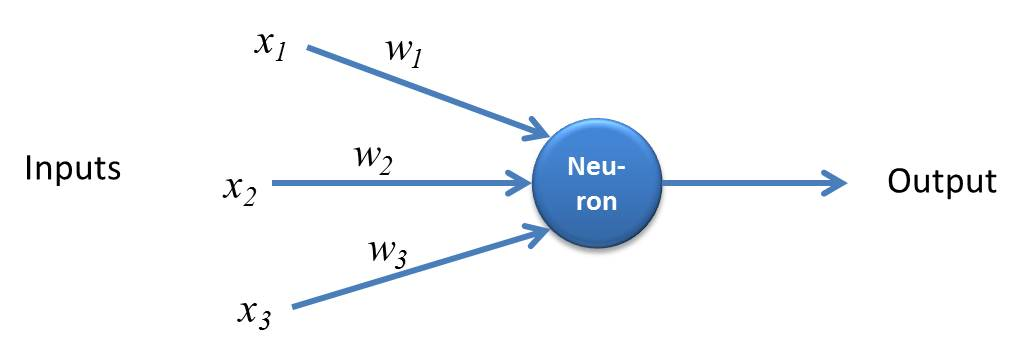
\includegraphics[width = 90mm]{immagini/Perceptron}
	\caption{Visualizzazione di un percettrone}
\end{figure}


Una rete con un solo percettrone è chiamata a singolo livello. Esistono poi le reti multistrato, sono reti che hanno minimo 3 nodi disposti su più livelli, figura 8:
\begin{itemize}
	\item livello input
	\item livello output 
	\item hidden layer: livelli intermedi tra input e output 
\end{itemize}


In questa rete ogni nodo, escluso il nodo di input, usa una funzione di attivazione non lineare per modellare il comportamento e assieme alla backpropagation vengono usate per allenare il modello.

\begin{figure}[h]
	\centering
	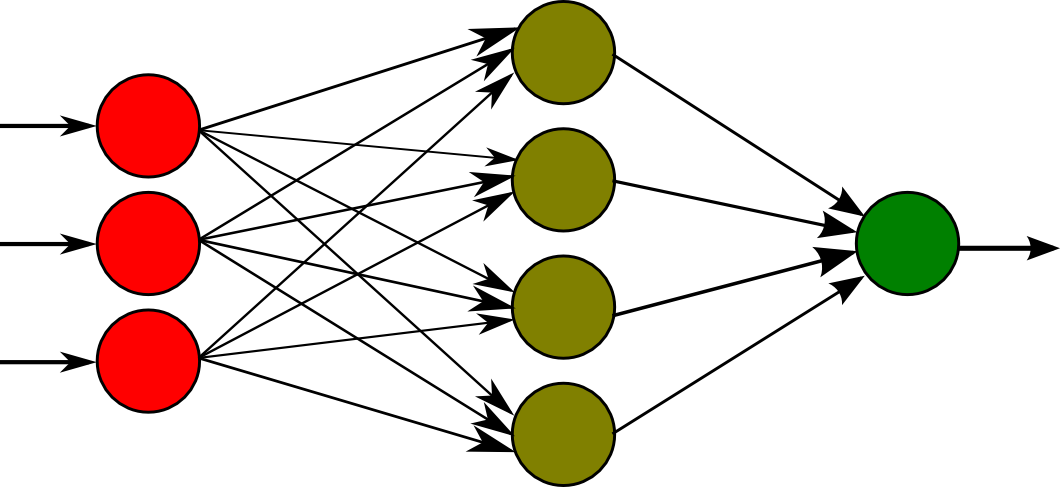
\includegraphics[width = 80mm]{immagini/Multilayer-Perceptron}
	\caption{Visualizzazione di una rete multistrato}
\end{figure}
La funzione di attivazione non fa altro che combinare l'input del neurone con i pesi e aggiungere un bias per produrre l'output.
Esistono diverse funzioni di attivazione:
\begin{itemize}
	\item Identity: $f(x) = x$
	\item Logistic: $f(x) = \frac{1}{1 + e^{-x}}$
	\item Tanh: $f(x) = tanh(x)$
	\item Relu: $f(x) = max(0, x)$
\end{itemize}
L'output $y$ viene calcolato nel seguente modo: 
\begin{equation}
y = ( \sum_{i=1}^{n}w_ix_i + b) = \Phi (w^{T}x + b)
\end{equation}
dove $w$ è il vettore di pesi, $x$ è il vettore di inputs, $b$ è il bias e $\Phi$ è la funzione di attivazione.

Il processo di addestramento del Multi-Layer Perceptron avviene mediante una continua regolazione dei pesi delle connessioni dopo ogni elaborazione. Questa regolazione si basa sull'errore nell'output. Questa regolazione continua dei pesi è un processo di apprendimento supervisionato chiamato ``backpropagation''.
Il processo continua fino a quando l'errore non raggiunge il valore più basso.
\subsection{Machine Learning con apprendimento\\ non supervisionato}
Nell’apprendimento non supervisionato, al contrario di quello supervisionato abbiamo dei dati senza etichetta o dati non strutturati. Le tecniche di apprendimento non supervisionato mirano ad estrarre, in modo automatico, della conoscenza a partire da basi di dati. Questo avviene senza una specifica conoscenza dei contenuti da analizzare. Un esempio tipico di questi algoritmi lo si ha nei motori di ricerca. Questi programmi, data una o più parole chiave, sono in grado di creare una lista di link rimandanti alle pagine che l'algoritmo di ricerca ritiene attinenti alla ricerca effettuata.

I principali algoritmi sono:
\begin{itemize}
	\item Clustering
	\item Regole di associazione
\end{itemize}
\subsection{Machine Learning con apprendimento per rinforzo}
Il terzo tipo di apprendimento automatico è l’apprendimento per rinforzo. L’obiettivo di questo tipo di apprendimento è quello di costruire un sistema che attraverso le interazioni con l’ambiente migliori le proprie performance.

Per poter migliorare le funzionalità del sistema vengono introdotti dei rinforzi, ovvero segnali di ricompensa.

Questo rinforzo non è dato dalle label (etichette) o dai valori corretti di verità, ma è una misurazione sulla qualità delle azioni intraprese dal sistema. Per questo motivo non può essere assimilato ad un apprendimento supervisionato.
Potremmo trovare questo tipo di apprendimento ad esempio nell’addestramento di un sistema per il gioco degli scacchi.

Inizialmente le mosse saranno del tutto casuali e senza una logica. Dal momento in cui il sistema riceverà dei feedback positivi, come ad esempio nel caso in cui mangi una pedina avversaria, allora riceverà un peso maggiore e conseguentemente un rinforzo positivo su quell’azione. Contrariamente in caso di azione negativa, il valore dei pesi su quell’azione andrà in decremento.

Conseguentemente a questi rinforzi, il sistema darà maggior peso alle mosse che gli hanno portato maggiori benefici e tenderà a replicare lo stesso comportamento su nuove mosse future.
\subsection{Machine Learning con apprendimento semi Supervisionato}
Può essere visto come un quarto tipo di apprendimento automatico. In questo caso, al contrario dell’apprendimento non supervisionato, abbiamo che di tutti i dati presenti nel training set, solo pochi di essi sono stati etichettati.
% 
%			CAPITOLO 2: Stato dell'arte
% 

\chapter{Dataset}


\section{Iris}


\section{Incidenti Stradali}





\section{Metodi per ridurre la Dimensionalità}



\subsection{PCA}
\subsection{TSNE}


% 
%			CAPITOLO 3: Tecnologie utilizzate
% 

\chapter{Esperimenti}
\label{cap3}



\section{Model Selection}

\subsection{Scelta degli Iperparametri}

\begin{equation}
x_i(n) = a_{i1}u_1(n) + a_{i2}u_2(n) + \cdots + a_{iJ}u_J(n) \, .
\label{eq:multimix}
\end{equation}

\subsection{Scalare i dati}


\section{Errore di Generalizzazione}
\label{sec:errore}


\subsection{Training}



\subsection{Cross Validation}



\section{Risultati Ottenuti}
\label{sec:risultati}


% 
%			CAPITOLO 4: Conclusioni e sviluppi futuri
% 
\section{Conclusioni}

Nelle conclusioni si tirano le somme di quanto realizzato, facendo un riassunto stringato del lavoro svolto. In particolare vanno dichiarati punti di forza e criticità della ricerca effettuata, nonché quali aspetti dello stato dell'arte siano stati superati dal lavoro in oggetto.

%
%			BIBLIOGRAFIA
%

\bibliographystyle{unsrt}
\bibliography{bibliografia}
\addcontentsline{toc}{chapter}{Bibliografia}


\end{document}


 